\documentclass{article}
\usepackage[margin=1in]{geometry}
\usepackage{../common}
\usepackage{../pagesetup}
\usepackage{tikz}
\usetikzlibrary{bayesnet}
% **** IF YOU WANT TO DEFINE ADDITIONAL MACROS FOR YOURSELF, PUT THEM HERE:

\nc{\wt}{\widetilde}
\nc{\CN}{\mathcal N}
\nc{\Cat}{\on{Cat}}
\nc{\ol}{\overline}
\nc{\one}{\mathbf{1}}
\newtheorem{thm}{Theorem}
\newenvironment{solution}{\begin{proof}[Solution]}{\end{proof}}

\algnewcommand\algorithmicinput{\textbf{Input:}}
\algnewcommand\Input{\item[\algorithmicinput]}
\algnewcommand\algorithmicoutput{\textbf{Output:}}
\algnewcommand\Output{\item[\algorithmicoutput]}
\algnewcommand\algorithmicinitialize{\textbf{Initialize:}}
\algnewcommand\Initialize{\item[\algorithmicinitialize]}

\begin{document}

\lecture{16}{November 1}{Sasha Rush}{ Denis Turcu,Xu Si,Jiayu Yao}{Variational Inference Part 2}

\subsection{Announcements} 
\begin{itemize}
\item T4 out, due 9/13 at 5pm
\item Exams available in office
\item OH - today 2:30-4pm (Wednesdays)
\item  Follow formatting for the abstract of the final project. There were many inconsistencies with the formatting requirements for the initial proposal.
\end{itemize} 

\subsection{Introduction}
Last class, we talked about variational inference. This class, we gonna talk about a very different type of VI. We also will talk about some other types of VI but will not go too much into the details.  \newline

Murphy's book, especially Chapter 22, covers many details on the theory side. The other text, Murphy referred as "The Monster", we put online as a textbook written by Michael Jordan.

\subsection{Bayesian GMM}
We are going to talk more about variational inference. We also put another reference online called VI: A Review for Statisticians \cite{BKM17}. It covers in great detail of Bayesian GMM, so let's write down that model:
\begin{center}
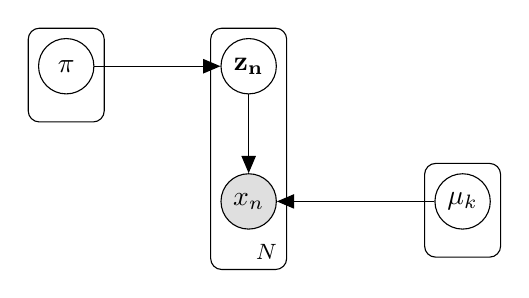
\begin{tikzpicture}

  % Define nodes
  \node[obs]                               (x) {$x_n$};
  \node[latent, above=of x, xshift=0cm]  (z) {$\mathbf{z_n}$};
  \node[latent, left=of z, xshift=-0.6cm] (pi) {$\pi$};
  \node[latent, right=2cm of x]            (mu) {$\mu_k$};

  % Connect the nodes
  \edge {z,mu}{x} ; %
  \edge {pi}{z} ; %

  % Plates
  \plate{}{(mu)}{}
 \plate {}{(pi)}{} 
  \plate {}{(z)(x)}{$N$} ;

\end{tikzpicture}
\end{center}
We assume:
\[ \mu_k \sim \mathcal{N}(0,\sig^2) \;\forall\;k \]
\[ z_n \sim Cat(\f{1}{k}, \dots,\f{1}{k}) \;\forall\; k\]
\[ x_n | z_n, \mu \sim \mathcal{N}(\mu_{z_n},1) \; \forall \; n. \]

Then we write:
\[ p(\{x_n\},\{z_n\},\mu) = p(\mu) \prod_n p(z_n) p(x_n|z_n,\mu). \]
And we get:
\[ p(x) = \int_{z,\mu} p(x,z,\mu) = \int p(\mu) \prod_n \sum_{z_n} p(z_n) p(x_n|z_n,\mu) \rd \mu. \]

{\em Variation setup}. 
Goal:\[ \min_{q\in EASY} KL(q||p) \] 
reverse KL.

We pick $EASY$ as mean field. 
\begin{center}
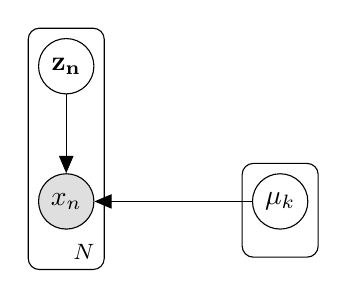
\begin{tikzpicture}

  % Define nodes
  \node[obs]                               (x) {$x_n$};
  \node[latent, above=of x, xshift=0cm]  (z) {$\mathbf{z_n}$};
  \node[latent, right=2cm of x]            (mu) {$\mu_k$};

  % Connect the nodes
  \edge {z,mu} {x} ; %

  % Plates
  \plate{}{(mu)}{}
  \plate {} {(z)(x)} {$N$} ;

\end{tikzpicture}
\end{center}
\begin{center}
p
\end{center}
 
\begin{center}
\begin{tikzpicture}

  % Define nodes
    \node[latent]            (mu) {$\mu_k$};
  \node[latent, left=of x, xshift=-1cm]  (z) {$\mathbf{z_n}$};


  % Plates
  \plate{}{(mu)}{}
  \plate {} {(z)}{} ;
\end{tikzpicture}
\end{center}

\begin{center}
q
\end{center}
Variational parametrization:

\[ q(\mu, z) = \prod_k q_k(\mu_k)\prod_n q_n(z_n). \]

\[ q_n(z_n;\lam_n^{z}) \hspace{2cm} Cat(\lam_n^z). \]
\[ q_k(\mu_k;\lam_k^{\mu}, \lam_k^{\sig^2}) \hspace{2cm} \mathcal{N}(\lam_k^{\mu}, \lam_k^{\sig^2}). \]
\[ \arg \min _{q\in EASY} KL(q||p) = \arg\min_\lam KL \left( \prod_k q_k(\mu_k;\lam_k^{\mu}, \lam_k^{\sig^2}) \prod_n q_n(z_n;\lam_n^{z})  \; || \;  p \right) \] \\ 



"When we do {\em mean field}?"

\[ q_i \sim \exp[ \E_{-q_i} \log(p(z,x)) ]\]

Brief interlude: coordinate ascent $\to$ CAVI (coordinates ascent variational inference). Doing each individual one at a time.
\begin{itemize}
\item Bound we are optimizing is non-convex.
\item This method is monotonically increasing.
\item Sensitive to initialization $\to$ common for random restarts.
\end{itemize}

\bigskip

Example, deriving the math for GMM can be useful to understand how it works and how we will do mean field updates. Start from the above, setup the problem:

\[ \mu_k \sim \mathcal{N}(0,\sig^2) \;\forall\;k \]
\[ z_n \sim Cat(\f{1}{k}, \dots,\f{1}{k}) \;\forall\; k\]
\[ x_n | z_n, \mu \sim \mathcal{N}(\mu_{z_n},1) \; \forall \; n \]

where we also have $\lam_n^z$ for hidden switch variable, and $\lam_k^m, \lam_k^{s^2}$ for the Gaussians.

\begin{align*}
q_n(z_n; \lam_n^z) &\propto exp[\E_{-q_n} \log (p(\mu,z,x))] \\
&\propto exp[\E_{-q_n} \log (p(x_n|z_n, \mu_{z_n}))] \\
&\propto exp[\E_{-q_n} - (x_n - \mu_{z_n})^2 / z] \\
&\propto exp[\E_{-q_n} (x_n\mu_{z_n} - \mu_{z_n}{}^2 / 2)]\\
&\propto exp[x_n \E_{-q_n}(\mu_{z_n}) - \E_{-q_n}(\mu_{z_n}{}^2) / 2]\\
\end{align*}


\begin{center}
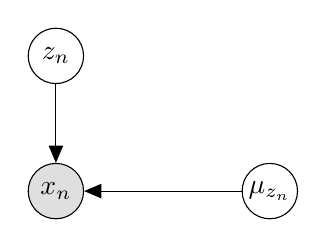
\begin{tikzpicture}

  % Define nodes
  \node[obs]                               (x) {$x_n$};
  \node[latent, above=of x, xshift=0cm]  (z) {$z_n$};
  \node[latent, right=2cm of x]            (mu) {$\mu_{z_n}$};

  % Connect the nodes
  \edge {z,mu} {x} ; %

\end{tikzpicture}
\end{center}

So we identify $ \E_{-q_n}(\mu_{z_n})$ with $\lam_{k=z_n}^m$ and $\E_{-q_n}(\mu_{z_n}{}^2)$ with $\lam_k^{s^2}$, and then we can write:

\begin{align*}
q_k(\mu_k; \lam_{k=z_n}^m, \lam_k^{s^2}) &\propto exp [\E_{-q_n} (\log p(\mu_k) + \sum_n \log p(x_n|z_n,\mu)] \\
&= -\mu_k{}^2 / (2 \sig^2) + \sum_n \E(\log p(x_n|z_n,\mu)) \\
&= -\mu_k{}^2 / (2 \sig^2) + \sum_n \E(z_{nk} (\log p(x_n|\mu_k)) \\
&= -\mu_k{}^2 / (2 \sig^2) + \sum_n \E_{-q_n}(z_{nk}) (\log p(x_n|\mu_k)) \\
&= -\mu_k{}^2 / (2 \sig^2) + \sum_n \lam_{nk}^z  (-(x_n - \mu_{z_n}))^2 / 2 + const. \\
&= (\sum_k \lam_{nk}^z x_n)\mu_k - (\f{\sig^2}{2} + \sum \lam_{nk}^z / 2) \mu_k{}^2 + const. 
\end{align*}

Then:
\[ q_k(\mu_k) = exp[ \tta ^T \phi - A + \dots ], \]
where $\tta_1 = \sum_n \lam_{nk}^z x_n, \; \tta_2 = -(\f{\sig^2}{2} + \sum \lam_{nk}^z / 2$) and $\phi_1 = \mu_k, \; \phi_2 = \mu_k{}^2$, as in GLM.

For normal distribution, we have:
\[ \lam_k^m = \f{\sum_n \lam_{nk}^z x_n}{1/\sig^2 + \sum_n \lam_{nk}^z}, \trm{ and } \lam_k^{s^2} = \f{1}{1/\sig^2 + \sum_n \lam_{nk}^z}. \]

\subsection{Exponential Family}

\[ p(z_j|z_{-j},x) = h(z_j) exp(\tta^T\phi(z_j) - A(\tta)), \]
where $\tta$ are function of $z_{-j}, x$. One nice case is {\em UGM}:

\begin{center}
\begin{tikzpicture}

  % Define nodes
  \node[latent]       (mid) {$z_j$};
  \node[latent, above=of mid, yshift=0.5cm]  (up) {};
  \node[latent, below=of mid, yshift=-0.5cm]  (below) {};
  \node[latent, left=of mid, xshift=-0.5cm]  (left) {};
  \node[latent, right=of mid, xshift=0.5cm]  (right) {};

  % Connect the nodes
  \edge[-] {up} {mid} ;
  \edge[-] {right} {mid} ;
  \edge[-] {below} {mid} ;
  \edge[-] {left} {mid} ;

\end{tikzpicture}
\end{center}
\begin{center}
blanket
\end{center}


\[ q(z) = \prod_j q(z_j)\]
\begin{align*}
q(z) &\propto exp[\E_{-q_j} \log p(z_j|z_{-j},x)] \\
&\propto exp[ \log(h) + \E(\tta)_{z_j}^T - \E (A(\tta))] \\
&\propto h(z_j) exp[\E(\tta)^T z_j]
\end{align*}

where $\E(\tta)^T$ are the natural parameters of the variational approximation \newline
\[\lambda_j = \E[\theta(z_{-j},x)]\]

\subsection{Latent Dirichlet Allocation}
\begin{itemize}
\item Widely used generative latent variable model
\item generative model set up
\begin{center}
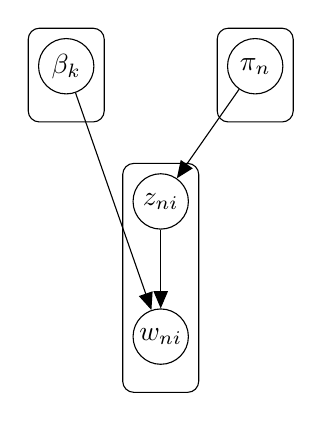
\begin{tikzpicture}

  % Define nodes
  \node[latent]                               (w) {$w_{ni}$};
  \node[latent, above=of w, xshift=0cm]  (z) {$z_{ni}$};
  \node[latent, above=of z, xshift=-1.2cm] (beta) {$\beta_k$};
  \node[latent, above=of z, xshift=1.2cm]            (pi) {$\pi_n$};

  % Connect the nodes
  \edge {z} {w} ; %
  \edge {beta} {w} ; %
  \edge {pi} {z} ; %

  % Plates
  \plate{}{(beta)}{}
 \plate {} {(pi)} {} 
  \plate {} {(z)(w)} {} ;

\end{tikzpicture}
\end{center}
where $\be_k \sim Dir(\eta)$, $\pi_n \sim Dir(\alpha)$, $z_{ni} \sim Cat(\pi_n)$, $w_{ni} \sim Cat(\be_{z_{ni}})$
\item Topic molding story: 
\begin{itemize}
\item $n$ - documents
\item $i$ - words
\item $\pi_n$ - document topic distribution
\item $\be_k$ - topic-word distribution
\item $z_{ni}$ - topic selected for word $i$ of document $n$ 
\item $w_{ni}$ - word selected for $ni$. 
\item $\lam_{ni}^z$ - probability for the topic of word $i$ in document $n$
\end{itemize}
 


\end{itemize}

\subsection{Demo}

\smallskip
We did an example iPython notebook (\href{https://github.com/harvard-ml-courses/cs281-demos/blob/master/TopicModeling.ipynb}{\texttt{TopicModeling.ipynb}}) in class.

\subsection{Exercise: Variational Bayes EM}

In lecture we discussed variational inference for Gaussian mixture models.\footnote{This section and exercise written by Jeffrey Cai.} As covered by the notes ``Variational Inference: A Review for Statisticians'' \cite{BKM17}, we have the following formal description of the update steps, where the notation is as follows:
\begin{itemize}
\item $z_i$ are the latent cluster labels with prior $\Cat(\frac{1}{K}, \dots, \frac{1}{K})$.
\item $y_i$ are the data.
\item $\mu_k$ are the latent cluster means with prior $\CN(0, \sigma^2)$.
\item $\wt{\mu}, \wt{\sigma}^2$ are variational parameters for $q(\mu_k) \sim \CN(\wt{\mu}_k, \wt{\sigma}^2_k)$.
\item $\wt{\alpha}$ are variational parameters for $q(z_i) \sim \Cat(\wt{\alpha}_i)$.
\end{itemize}

\begin{algorithm}
    \caption{CAVI for a Gaussian mixture model}
    \label{alg:cavigmm}
    \begin{algorithmic}[1]
        \Input{Data $y_1, \dots, y_n$, number of components $K$, prior variance of component means $\sigma^2$}
        \Output{Variational densities $q(\mu_k) \sim \CN(\wt{\mu}_k, \wt{\sigma}^2_k)$ and $q(z_i) \sim \Cat(\wt{\alpha}_i)$}
        \While{the ELBO has not converged}
            \For{$i \in \{1, \dots, n\}$}
                \State \textbf{Set} $\wt{\alpha}_{ik} \propto \exp\{ \wt{\mu}_k y_i - \frac{1}{2} (\wt{\mu}_k^2 + \wt{\sigma}_k^2) \}$
            \EndFor
            \For{$k \in \{1, \ldots, K\}$}
                \State \textbf{Set} $\displaystyle \wt{\mu}_k \gets \frac{\sum_i \wt{\alpha}_{ik} y_i}{1/\sigma^2 + \sum_i \wt{\alpha}_{ik}}$
                \State \textbf{Set} $\displaystyle \wt{\sigma}^2_k \gets \frac{1}{1/\sigma^2 + \sum_i \wt{\alpha}_{ik}}$
            \EndFor
            \State \textbf{Compute} $\on{ELBO}(\wt{\mu}, \wt{\sigma}^2, \wt{\alpha})$
        \EndWhile
        \State \textbf{Return} $q(\wt{\mu}, \wt{\sigma}^2, \wt{\alpha})$
    \end{algorithmic}
\end{algorithm}

In fact, this algorithm can be seen as a special case of the \emph{variational Bayes EM} algorithm. This algorithm is really only tractable for conjugate-exponential models, and we shall state the result for that case below. The result is found in \cite{Beal03}.

\begin{thm}[Variational Bayes EM for Conjugate-Exponential Models]\label{thm:vbem}
Suppose we have a model with parameters $\mu$ giving rise to an i.i.d. data set $y = \{y_1, \dots, y_n\}$ with corresponding hidden variables $z = \{z_1, \dots, z_n\}$. Suppose further that the complete-data likelihood is in the exponential family:
\[ p(y_i, z_i \given \mu) \propto f(y_i, z_i) \exp\left[ \theta(\mu)^\top u(y_i, z_i) \right], \]
and that the parameter prior is conjugate to the complete-data likelihood:
\[ p(\mu \given \eta, \nu) \propto g(\mu)^\eta \exp\left[ \theta(\mu)^\top \nu \right] \]
where $\eta, \nu$ are hyperparameters, and ``conjugate'' means that the posterior
\[ p(\mu \given \eta', \nu') \propto p(\mu \given \eta, \nu) p(y, z \given \mu) \]
has the same parametric form as the prior.

Suppose our variational family consists of factored distributions
\[ q(z, \mu) = q(\mu) \cdot \prod_i q(z_i). \]
Then iterating VBE and VBE steps, given below, causes the ELBO to converge to a local maximum.

\emph{VBE Step}: Given $q(\mu)$ from the previous epoch, define $q(z)$ for the VBM step by:
\begin{align*}
q(z_i) &\propto f(y_i, z_i) \exp\left[ \ol{\theta}^\top u(y_i, z_i) \right] \\
\text{where }\ol{\theta} &= E_{q(\mu)}[\theta(\mu)].
\end{align*}

\emph{VBM Step}: Given $q(z)$ from the VBE step, define $q(\mu)$ for the next epoch by:
\begin{align*}
q(\mu) &\propto g(\mu)^{\wt{\eta}} \exp\left[ \theta(\mu)^\top \wt{\nu} \right] \\
\text{where }\wt{\eta} &= \eta + n \\
\wt{\nu} &= \nu + \sum_{i=1}^n \ol{u}(y_i) \\
\text{where }\ol{u}(y_i) &= E_{q(z_i)}[u(y_i, z_i)].
\end{align*}
\end{thm}

\begin{exercise}
Here you will show the claim that the ``CAVI for a Gaussian mixture model'' algorithm is in fact a special case of VBEM for conjugate-exponential models.

(a) Express the complete data likelihood $p(y_i, z_i \given \mu)$ for the Gaussian mixture model in exponential family form. That is, give the natural parameters $\theta(\mu)$, the sufficient statistics $u(y_i, z_i)$, and the function $f(y_i, z_i)$. \emph{Hint:} There should be $2K+1$ sufficient statistics.

(b) Express the parameter prior in exponential family form. (Note that the natural parameters $\theta(\mu)$ should be the same as those you derived in (a).)

(c) Assume that from the previous epoch, $q(\mu_k) \sim \CN(\wt{\mu}_k, \wt{\sigma}^2_k)$. Show that after applying the VBE updates in Theorem~\ref{thm:vbem}, one obtains $q(z_i) \sim \Cat(\wt{\alpha}_i)$ where the resulting $\wt{\alpha}_i$ is the same as the Algorithm~\ref{alg:cavigmm} update.

(d) Assume that from the VBE step, $q(z_i) \sim \Cat(\wt{\alpha}_i)$. Show that after applying the VBM updates in Theorem~\ref{thm:vbem}, one obtains $q(\mu_k) \sim \CN(\wt{\mu}_k, \wt{\sigma}^2_k)$ where the resulting $\wt{\mu}_k, \wt{\sigma}^2_k$ is the same as the Algorithm~\ref{alg:cavigmm} update.
\end{exercise}

\begin{solution}
\renewcommand\arraystretch{1.5}
(a) We have,
\begin{align*}
p(y_i, z_i \given \mu) &= \frac{1}{K} \cdot \frac{1}{\sqrt{2\pi}} \cdot \exp\left[ -\frac{1}{2} (y_i - \mu_{z_i})^2 \right] \\
&= \frac{1}{\sqrt{2\pi} K} \exp\left[ -\frac{1}{2} y_i^2 + \sum_{k=1}^K \one_{z_i = k} \left(y_i \mu_k - \frac{1}{2} \mu_k^2 \right) \right].
\end{align*}
From this we deduce:
\[
\theta(\mu) = \begin{bmatrix} (-\mu_k^2/2)_{k=1}^K \\ (\mu_k)_{k=1}^K \\ -1/2 \end{bmatrix}
\qquad
u(x_i, y_i) = \begin{bmatrix} (\one_{z_i = k})_{k=1}^K \\ (\one_{z_i = k}\, y_i)_{k=1}^K \\ y_i^2 \end{bmatrix}
\qquad
f(x_i, y_i) = 1.
\]

(b) We have,
\[ p(\theta) = \prod_k p(\theta_k) = \left( \frac{1}{\sqrt{2\pi}\sigma} \right)^K \exp\left[ \sum_{k=1}^K \left( -\frac{\theta_k^2}{2\sigma^2} \right) \right]. \]
Consequently,
\[
\nu = \begin{bmatrix} (1/\sigma^2)_{k=1}^K \\ (0)_{k=1}^K \\ 0 \end{bmatrix}.
\]

(c) We have,
\[
\ol{\theta} = E_{q(\mu)}[\theta(\mu)] = \begin{bmatrix} (-E_{q(\mu)}[\mu_k^2]/2)_{k=1}^K \\ (E_{q(\mu)}[\mu_k])_{k=1}^K \\ -1/2 \end{bmatrix} = \begin{bmatrix} ((\wt{\mu}_k^2 + \wt{\sigma}_k^2)/2)_{k=1}^K \\ (\wt{\mu}_k)_{k=1}^K \\ -1/2 \end{bmatrix}
\]
and therefore
\begin{align*}
q(z_i) &\propto \exp\left[ -\frac{1}{2} \sum_{k=1}^K \one_{z_i=k} ( \wt{\mu}_k^2 + \wt{\sigma}_k^2 ) + \sum_{k=1}^K \one_{z_i=k}\, y_i \wt{\mu}_k - \frac{1}{2}y_i^2 \right] \\
&= \exp\left[ -\frac{1}{2} (\wt{\mu}_{z_i}^2 + \wt{\sigma}_{z_i}^2) + y_{z_i} \wt{\mu}_{z_i} + \text{const.} \right]
\end{align*}
which is the desired form.

(d) We have,
\[
\ol{u}(y_i) = \begin{bmatrix} (\wt{\alpha}_{ik})_{k=1}^K \\ (\wt{\alpha}_{ik}y_i)_{k=1}^K \\ y_i^2 \end{bmatrix}
\]
and therefore
\[
\ol{\nu} = \nu + \sum_{i=1}^n \ol{u}(y_i) = \begin{bmatrix} (\frac{1}{\sigma^2} + \sum_{i=1}^N \wt{\alpha}_{ik})_{k=1}^K \\ (\sum_{i=1}^N \wt{\alpha}_{ik} y_i)_{k=1}^K \\ y_i^2 \end{bmatrix}
\]
and then
\begin{align*}
q(\mu) &\propto \exp\left[ \sum_{k=1}^K \left( -\frac{1}{2} \mu_k^2 \left(\frac{1}{\sigma^2} + \sum_{i=1}^N \wt{\alpha}_{ik}\right) + \mu_k \sum_{i=1}^N \wt{\alpha}_{ik} y_i \right) - \frac{1}{2} y_i^2 \right] \\
&= \exp\left[ \sum_{k=1}^K -\frac{1}{2\wt{\sigma}^2_k} (\mu_k^2 - 2\wt{\mu}_k \mu_k) + \text{const.} \right] \\
&= \exp\left[ \sum_{k=1}^K -\frac{(\mu_k - \wt{\mu}_k)^2}{2\wt{\sigma}^2_k} + \text{const.} \right]
\end{align*}
where $\wt{\sigma}^2_k = (\sigma^{-2} + \sum_i \wt{\alpha}_{ik})^{-1}$ and $\wt{\mu}_k = \wt{\sigma}^2_k \sum_i \wt{\alpha}_{ik} y_i$ are the desired parameter updates, and in the last step we completed the square by pulling a missing term from the constant. Hence $q(\mu)$ has the desired form.
\end{solution}

\begin{thebibliography}{99}
\bibitem[Beal03]{Beal03}
  Beal, M. Variational methods for approximate Bayesian inference. PhD thesis, University of London, 2003.
\bibitem[BKM17]{BKM17}
  Blei, M., Kucukelbir, A., and McAuliffe, J. Variational Inference: A Review for Statisticians. \textit{ Journal of the American Statistical Association}, 112(518), 2017.
\end{thebibliography}

\end{document}